\documentclass[12pt,final]{rureport}

\begin{document} % this tells the compiler that it is time to make
                 % text to print instead of just getting ready.
\maketitle  % make a title page from the Title, Date, and Author
\listoffixmes

\section{Inngangur}
	Reglunarkerfi er að finna alls staðar í kringum okkur, allt frá flugvélum til hraðastýringa í bílum. Notagildi kerfanna er mismunandi og fer alfarið eftir aðstæðum. Þeim má beyta á ýmsa vegu, til dæmis í að halda kerfi stöðugu eða stjórna síbreytilegu ástandi kerfisins.
	
	Markmið þessa verkefnis er að hanna PID reglunarkerfi til að halda vatnshæð í tanki stöðugri. Fyrri hluti verkefnisins felst í að finna viðeigandi stærðfræðilíkan fyrir kerfið á formi yfirfærslufalla. Með mælingum á svörun kerfisins má finna stuðla yfirfærlsufallana. Síðan skal nota Simulink til bera saman þær svaranir sem fengnar voru með líkaninu við prófun á kerfinu.
	
	Í seinni liðnum skal beita PI reglunarkerfi þannig að æstæða skekkja kerfisins verði núll, þegar innmerkinu er breytt úr föstu gildi í annað fast gildi. Einnig skal athuga hvort hægt sé að auka viðbragðstíma kerfisins með því að nota PID stýringu.


\section{Framkvæmd}
	\subsection{Fyrri hluti: P Stýring}
	\subsubsection{Yfirfærsluföll}
	\begin{figure}[h]
		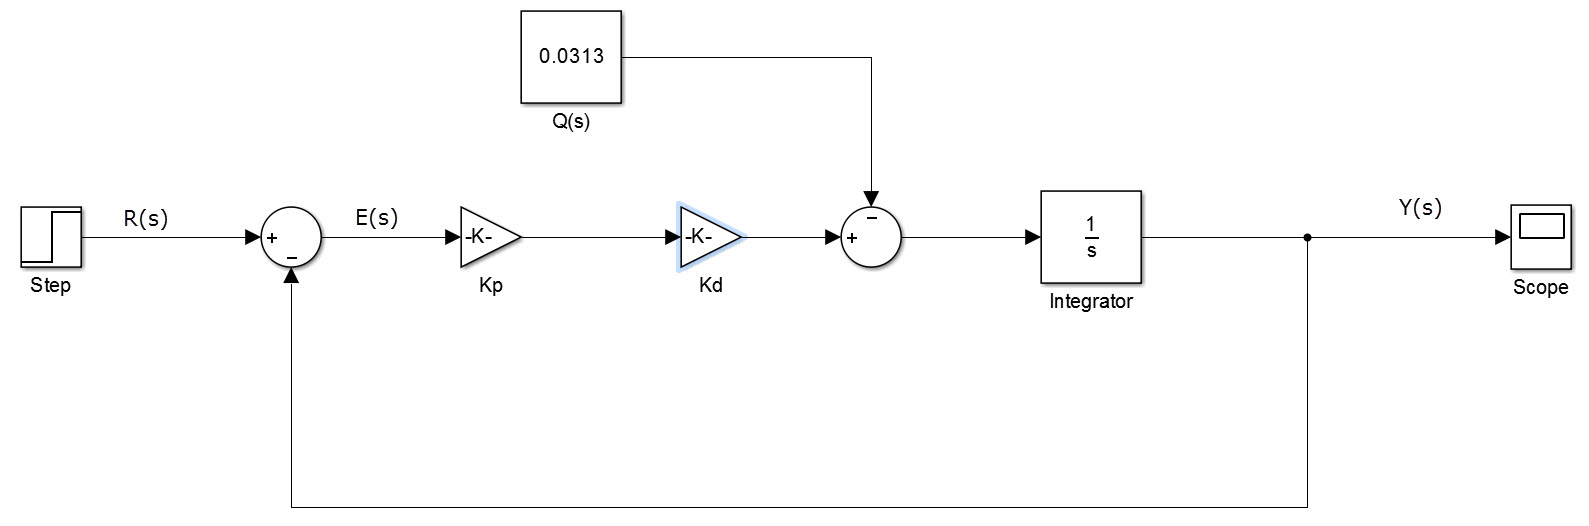
\includegraphics[width=\linewidth]{Block_diagram.jpg}
		\caption{Kassarit af kerfinu}
		\label{fig:blockrit}
	\end{figure}
	\hspace{-21pt}
	Eftirfarandi yfirfærsluföll eru fengin með því að nota reglu Mason á kassarit sem sjá má á mynd \ref{fig:blockrit}.\\
	Yfirfærlsufall lokuðu rásarinnar án truflunar:
	\[
		T_L(s) = \frac{R(s)}{Y(s)} = \frac{\frac{1 \cdot K_D K_P}{s}}{1 + \frac{1 \cdot K_D K_P}{s}} = \frac{K_D K_P}{s + K_D K_P}
	\]
	Yfirfærslufall rásarinnar út frá truflun:
	\[
		T_Q(s) = {Q(s) \over Y(s)} = \frac{{Q(s) \cdot 1 \over s}}{s + K_D K_P} = {Q(s) \over s^2 + s K_D K_P}
	\]
	Heildaryfirfærslufall rásarinnar er því:
	\[
		T(s) = T_L(s) - T_Q(s) = \frac{K_D K_P}{s + K_D K_P} - {Q(s) \over s^2 + s K_D K_P} = \frac{s K_P K_D - Q(s)}{s^2 + s K_D K_P}
	\]
	
	Innmerkið, $R(s)$, er óskgildi á vatnshæð tanksins, sem er stjórnað af okkur. Útmerkið $Y(s)$ er raungildi vatnshæðarinnar sem samanstendur af afkastagetu dælunnar og leka, sem við köllum $Q(s)$, sbr. mynd \ref{fig:blockrit}. Útmerkið $Y(s)$ er fundið með því að heilda nettó flæðið í tankinn, þ.e. flæðið inn í tankinn frá dælunni, en það verður að draga bakflæðið (lekann) frá því.
	
	\subsubsection{Bakflæði og dælustuðull}
	\begin{figure}[h]
		\centering
		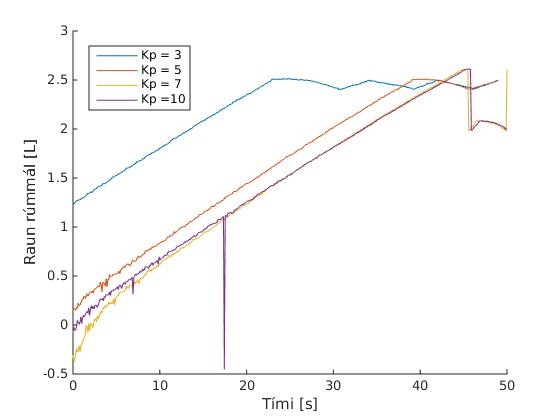
\includegraphics[scale=0.7]{sys_nofeedback.jpg}
		\caption{Kerfið án bakverkunar}
		\label{fig:nofeedback}
	\end{figure}
	
	Kerfið var skoðað án bakverkunar, sbr. mynd \ref{fig:nofeedback}, til að finna bakflæðið úr tankinum.\\ Upphaflega var óskgildið $2L$ og lækkað í $1L$ á meðan stýrispennan var stillt á $5V$.
	
	Við hermdum kerfið án bakverkunar og fengum þá rampmerki sem heldur áfram að vaxa út í hið óendanlega.
	

	\begin{figure}[]
		\centering
		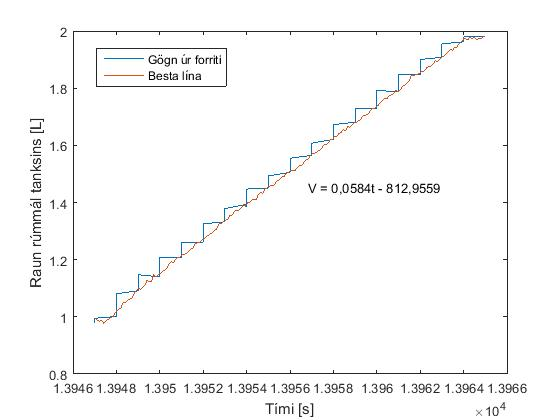
\includegraphics[scale=0.7]{pump.jpg}
		\caption{Rúmmál vatns í efri tank sem fall af tíma, dælustuðull}
		\label{fig:pump}
	\end{figure}
	
	Til að finna dælufastann var óskgildi sett sem $1L$ og hækkað í $2L$, stýrispennan var stillt á $5V$, sbr. mynd \ref{fig:pump}.
	
	Gögnin voru meðhöndluð með Matlab, notuð voru innbyggðu föllin polyval og polyfit til að finna bestu línu gagnanna. Bakflæðisstuðull kerfisins fengum við að væri $0.0313$, sbr. mynd \ref{fig:leki}. Stuðullinn afkastagetu dælunnar fengum við að sé $0.0584$ þegar stýrispenna er $5V$, sbr. mynd \ref{fig:pump}, sem gefur $0.0117$ fyrir hvert $V$ sem stýrispennan er.
	
	\begin{figure}[]
		\centering
		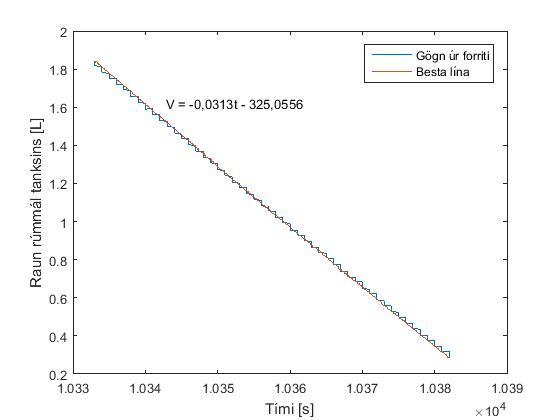
\includegraphics[scale=0.7]{leki.jpg}
		\caption{Rúmmál vatns í efri tank sem fall af tíma, bakflæðistuðull}
		\label{fig:leki}
	\end{figure}
	
	Við bjuggum til módel, sbr. mynd \ref{fig:blockrit}, sem hermir eftir hegðun kerfisins með mismundandi gildum á mögnunarstuðlinum Kp, sbr. mynd \ref{fig:feedback}, með og án bakverkunar. Við notuðum $Q(s) = 0.0313$ og $Kd = 0.0117$. Óskgildið var $2.5L$ og stýrispennan $5V$.
	
	\begin{figure}[]
		\centering
		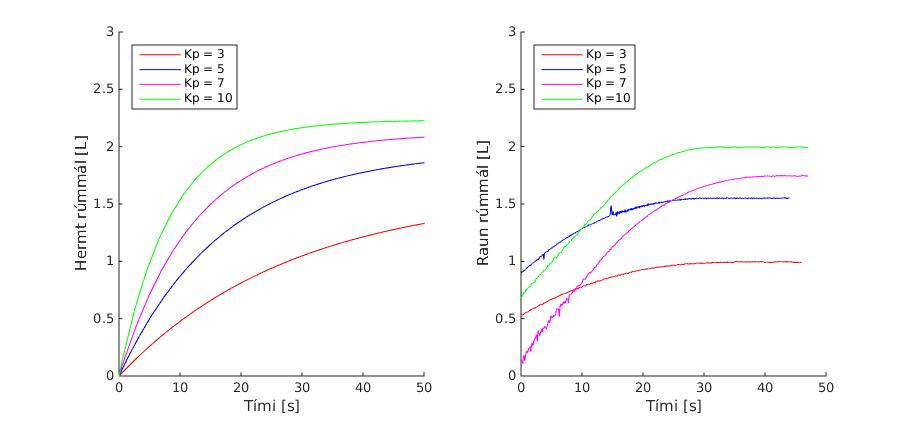
\includegraphics[width=\linewidth]{Kp_test_feedback.jpg}
		\caption{Samanburður á hermdu gildum og raungildum með bakverkun}
		\label{fig:feedback}
	\end{figure}
	
	\subsection{Seinni hluti: PI/PID Stýring}
	\subsubsection{Val á mögnun og heildunartíma}
	Til að finna hæfilegt gildi á $K_P$ og $T_D$ prófuðum við okkur áfram þangað til við fengum gildi sem okkur leist vel á.
	Við prófanir með mismunandi heildunartíma tókum við eftir því að yfirskotið jókst ef $T_i$ var sett of hátt, auk þess fór æstæða skekkjan $e_{ss}$ að aukast umfram það sem við vildum fá og varð óstöðug ef $T_i < 1$.
	
	Eftir að hafa skoðað nokkur gildi fannst okkur eðlilegast að hafa gildið á $T_i$ eins lágt og við kæmumst upp með, án þess að settíminn væri of mikill eða æstæða skekkjan óstöðug. Því prófuðum við okkur áfram með gildi kringum $T_i = 1$.
	
	\begin{figure}[h!]
		\centering
		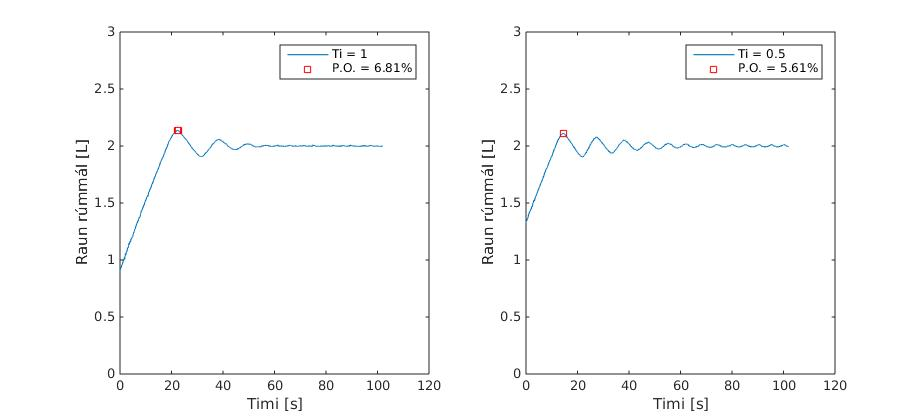
\includegraphics[width=\linewidth]{sys_intTime_best.jpg}
		\caption{Tekur langan tíma fyrir æstæða skekkju $e_{ss} \rightarrow 0$ þegar $T_i < 1$}
		\label{fig:intTime}
	\end{figure}
	
	Yfirskotið fyrir $T_i = 0.5$ fengum við að væri $P.O. = 5.61\%$, sbr. mynd \ref{fig:intTime}, en þar sem æstæða skekkjan var orðin of mikil ákváðum við frekar að láta reyna á hærri gildi. 
	
	Eins og áður var nefnt hækkar yfirskotið eftir því sem $T_i$ er hækkað, því ákváðum við nýta okkur þau gildi sem við fengum fyrir $T_i = 1$. Það gaf mjög litla æstæða skekkju og ásættanlegt yfirskot, en yfirskotið varð að vísu $P.O. = 6.81\%$, sbr. mynd \ref{fig:intTime}, sem er vissulega ekki minna en $5\%$ en æstæða skekkjan endaði í $\pm 0.01$.
	
	Við prófuðum einnig að setja $T_i$ sem $0.9$, $0.8$ og $0.7$ til að hafa yfirskotið sem minnst, en í öllum tilvikum fannst okkur æstæða skekkjan of mikil, því ákváðum við, eins og áður var tekið fram, að nota $T_i = 1$.
	
	\subsubsection{PID stýring}
	\begin{figure}[]
		\centering
		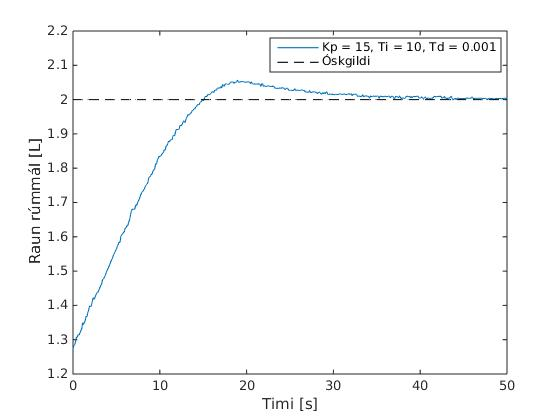
\includegraphics[scale=0.7]{sys_withdifftime.jpg}
		\caption{PID stýring: $K_P = 15$, $T_i  = 10$ og $T_d = 0.001$}
		\label{fig:difftime}
	\end{figure}
	Til að finna hæfilegan diffurtíma prófuðum við okkur enn og aftur áfram með því að breyta stuðlunum og sjá hvaða áhrif þeir hafa á kerfið. Fræðilega séð ætti yfirskot og settími að minnka þegar diffurtíminn er aukinn, skv. töflu 7.6 í námsbók, Modern Control Systems (Richard C. Dorf og Robert H. Bishop). Hins vegar verður kerfið virkilega óstöðugt ef diffurtíminn er aukinn um of, og mikið suð kemur í innmerkið.
	
	Eftir ítrekaðar tilraunir ákváðum við að best væri að hafa diffurtímann mjög lítinn þannig að hann hefði sem minnst áhrif á innmerkið og kerfið í heild sinni.
	
	Ekki er hægt að segja að viðbragðshraðinn aukist mikið við að hækka diffurtímann. Settími og ristími er mjög svipaður, u.þ.b. $20\,sek$ hvor, hvort sem notaður er diffurtími eða ekki, sbr. myndir \ref{fig:intTime} og \ref{fig:difftime}. Kerfið virðist hins vegar mun stöðugra þegar einhver diffurtími er kominn í kerfið og mun minna um sveiflur kringum óskgildið.
	
	Eftir töluverðar tilraunir með mismunandi stuðla ákváðum við að okkur þætti kerfið koma best út með stuðlana $K_P = 15$, $T_i = 10$ og $T_d = 0.001$ og sjá má hvernig það kom út á mynd \ref{fig:difftime}.

	\pagebreak	

%--------------------------------------------------------------------
%	Það má taka út appendixinn (það sem er hér fyrir neðan) ef ykkur
%	finnst þessi hluti óþarfur
%--------------------------------------------------------------------
\appendix
\section{Viðauki}
	\listoffigures

%\printbibliography
\end{document} % this tells the compiler that we are done

